\documentclass{article}
\usepackage{spconf,amsmath,graphicx,amssymb,cite,booktabs,url}
\usepackage{tikz}
\usetikzlibrary{positioning, shapes.geometric}
\usetikzlibrary{calc}

% Example definitions.
% ––––––––––
\def\x{{\mathbf x}}
\def\L{{\cal L}}

\newcommand{\eegtrans}{EEGXF}

% Title.
% ——
\title{On the Interplay of Temporal Context and Model Architecture for Naturalistic EEG Decoding}

% Author.
% ------
\name{First Author, Second Author, Third Author}
\address{Department of Computer Science, Your Institution \\
         Email: author1@domain.com, author2@domain.com, author3@domain.com}

\begin{document}
%
\maketitle
%
% \begin{abstract}
% We revisit the problem of EEG decoding under naturalistic stimulation and examine how varying the temporal context affects the performance of different neural architectures. Using the Healthy Brain Network dataset, we evaluate convolutional, recurrent, attention-based, and state space models on a movie classification task with EEG recordings. 
% We conduct a large-scale comparison of five model architectures (CNN, LSTM, Transformer, \eegtrans, S5) across segment lengths from 8s to 256s on a 4-class naturalistic EEG decoding task. While CNNs are competitive at short segments, structured state space models (SSMs), particularly S5, dominate in accuracy and training efficiency at longer durations. In subject-mixed splits, S5 reaches near-perfect accuracy at 256s. However, cross-frequency and subject-independent evaluations reveal significant performance drops, highlighting critical challenges in EEG generalization. We provide detailed comparisons of accuracy vs. efficiency and offer insights into model robustness across frequency and subject domains.
% In contrast to prior work where CNNs or Transformers dominate, we find that structured state space models (S5 in particular) consistently outperform across all segment lengths, achieving both higher accuracy and greater efficiency. We also identify a strong synergy between model type and segment duration: while CNNs perform adequately on short segments, only models with long-range sequence capacity generalize to longer temporal contexts. We release all code, models, and logs to support reproducibility and future benchmarking.
% \end{abstract}

\begin{abstract}
We investigate how model architecture and temporal context interact in naturalistic EEG decoding. Using the Healthy Brain Network dataset, we benchmark five architectures, CNN, LSTM, Transformer, \eegtrans (a modernized EEG Transformer), and S5 (a structured state space model), on a 4-class movie classification task across segment lengths from 8s to 256s. While CNNs perform well on short segments, S5 consistently outperforms in accuracy and training efficiency, particularly at longer durations. In subject-mixed splits, it reaches near-perfect accuracy on 256s segments, demonstrating its capacity for long-range temporal modeling. 
%S5 consistently outperforms in both accuracy and training efficiency at longer durations, reaching near-perfect accuracy at 256s in subject-mixed splits.

To assess real-world generalization, we conduct zero-shot cross-frequency evaluations and leave-one-subject-out (LOSO) testing. These reveal substantial performance drops, especially for S5, highlighting the challenge of subject-independent and frequency-robust EEG decoding. We also compare model efficiency and robustness, showing that S5 offers unmatched speed while \eegtrans is more stable across sampling rates. Our results provide practical insights for selecting EEG models under different generalization and efficiency constraints. We release all code, pretrained models, and training logs to ensure full reproducibility.
\end{abstract}


%
\begin{IEEEkeywords}
EEG decoding, state space models, S4, S5, Transformers, deep learning, naturalistic stimuli
\end{IEEEkeywords}
%


\section{Introduction}
\label{sec:intro}

Decoding brain activity from EEG during naturalistic tasks is a challenging and underexplored problem. Unlike trial-based paradigms, naturalistic stimuli like movie-watching evoke rich and temporally extended neural responses, requiring models that can capture long-range dependencies \cite{shirazi2024hbn}. Modern EEG datasets such as Healthy Brain Network (HBN) span minutes of continuous, noisy recordings across multiple conditions, highlighting the need for scalable, robust decoding methods.

Traditional architectures, CNNs, RNNs, and Transformers each have trade-offs. CNNs operate over fixed receptive fields and lack temporal flexibility \cite{roy2019deep}. LSTMs suffer from vanishing gradients and inefficiency over long sequences. Transformers provide global attention but scale quadratically in time and memory \cite{vaswani2017attention}. Structured State Space Models (SSMs), including S4 \cite{gu2022efficientlymodelinglongsequences} and its successor S5 \cite{gu2023mamba}, offer an alternative with near-linear time complexity and strong sequence modeling capabilities.

We hypothesize that sequence models like S5 and Transformers benefit more from long EEG segments than local models like CNNs. To test this, we benchmark five architectures—CNN, LSTM, Transformer, S4, and S5—on a 4-class movie classification task using HBN data, across segments from 8s to 256s. To ensure a strong baseline, we also develop and benchmark against \eegtrans, a modernized Transformer baseline incorporating best practices for EEG analysis.

Our evaluation spans subject-mixed and subject-independent scenarios, including a novel cross-frequency generalization test and a full leave-one-subject-out (LOSO) study. We find that S5 achieves near-perfect accuracy in subject-mixed splits and trains over 12× faster than Transformers, but suffers greater performance degradation under distributional shifts. These results highlight critical trade-offs between accuracy, speed, and robustness in real-world EEG decoding.

\paragraph*{Our Contributions}
\begin{itemize}
  \item We present the first systematic evaluation of five neural architectures across EEG segment lengths from 8s to 256s, revealing how temporal context interacts with model capacity.
  \item We introduce \eegtrans, a modernized Transformer baseline for EEG decoding, and benchmark it against CNNs, SSMs, and traditional Transformers.
  \item We evaluate generalization using two robust tests: (1) cross-frequency zero-shot inference with FIR and FFT downsampling; and (2) leave-one-subject-out (LOSO) subject transfer.
  \item We reveal a critical performance-robustness trade-off: S5 offers state-of-the-art speed and accuracy but is sensitive to distributional shifts, whereas \eegtrans provides greater robustness at a higher computational cost.
  % \item We show that while S5 offers unmatched speed and accuracy in subject-mixed setups, it is less robust than \eegtrans under frequency shifts and cross-subject generalization — a critical insight for practical EEG modeling.
\end{itemize}
% (Same as before, but you may want to add S5 if space allows or cite Mamba)
\section{Related Work}
\label{sec:related}

We build on recent advances in long-range sequence modeling to study how architecture and temporal context interact in naturalistic EEG decoding. Our work differs by combining model ablation, frequency robustness, and subject-transfer evaluation in one unified framework.

\subsection{Deep Learning for EEG Decoding}

CNNs have been widely adopted for EEG decoding, but their limited receptive fields often hinder the modeling of long-range dependencies \cite{roy2019deep,schirrmeister2017deep}. To address this, Transformer architectures have been introduced, leveraging self-attention to capture global dependencies. For instance, the EEG Conformer \cite{song2023eeg} integrates convolutional layers with Transformer modules to encapsulate both local and global features in a unified EEG classification framework. It also supports brain-topography visualization for interpretability. Hybrid models like the DB-Conformer \cite{wang2024dbconformer} employ a dual-branch design to model temporal and spatial features in parallel.

More broadly, the Transformer family has made significant inroads into BCI applications \cite{abibullaev2023transformerreview}. A recent survey outlines the promise and challenges of Transformers in EEG decoding, including motor imagery, emotion recognition, sleep staging, and speech reconstruction. These models benefit from temporal modeling and scale well with data, but face limitations in efficiency, interpretability, and training data requirements. This has motivated exploration of alternative architectures such as structured state space models (SSMs), which aim to preserve long-range modeling capabilities while improving computational efficiency. Other work has explored combining S4 with graph neural networks (GNNs) to model both temporal and spatial dynamics simultaneously \cite{tang2023graphs4mer}.

\subsection*{State Space Models in EEG}
Structured State Space Models (SSMs) such as S4 \cite{gu2022efficientlymodelinglongsequences} and its diagonalized successor S5 \cite{gu2023mamba} have shown strong performance in long-range sequence modeling. Recent works have begun applying SSMs to EEG:

\textbf{EEGMamba} \cite{wang2025eegmamba} introduces a foundation model trained on over 16,000 hours of EEG using a bidirectional Mamba encoder and masked patch prediction, achieving strong results across six tasks.

\textbf{DrowzEE-G-Mamba} \cite{siddhad2024drowzee} combines convolutional and Mamba blocks for driver drowsiness detection, improving performance on the SEED-VIG dataset through channel-shuffling and lightweight design.

\textbf{EEG-SSM} \cite{tran2024eegssm} proposes a model for dementia detection that jointly models temporal and spectral components of EEG signals. The approach significantly improves classification accuracy across varying temporal resolutions, reaching 91\% accuracy in a 3-class dementia classification task.

\textbf{DG-Mamba} \cite{li2025dgmamba} integrates Mamba with dynamic graph neural networks for efficient EEG event detection. It reduces training time and memory usage substantially while achieving strong results on seizure detection and sleep classification.

In contrast, our study focuses on segment-level classification in naturalistic EEG using S5 and baselines under a unified experimental protocol. While prior work demonstrates the flexibility of SSMs across various domains, we conduct the first detailed comparison of S5 to multiple architectures in terms of segment duration scaling, cross-frequency generalization, and LOSO subject transfer.

% BibTeX entries to be added:
% - EEGMamba
% - DrowzEE-G-Mamba
% - EEG-SSM (Tran et al. 2024)
% - DG-Mamba (Li et al. 2025)

\section{Dataset and Preprocessing}
\label{sec:data}

% (Same as before, but optionally update to reflect 40+ subjects and multiple segment lengths)

We utilize EEG data from the Healthy Brain Network (HBN) initiative \cite{shirazi2024hbn}. Specifically, we use recordings from the movie-watching tasks, %where participants viewed "Despicable Me," "Diary of a Wimpy Kid," and "The Present."
where participants viewed "Despicable Me," "Diary of a Wimpy Kid," "The Present," and a resting-state baseline.

The raw EEG data was downsampled to 250 Hz, and the first 64 channels were selected for consistency. Our preprocessing pipeline consisted of:
\begin{enumerate}
    \item \textbf{Filtering:} A 1-50 Hz bandpass filter.
    \item \textbf{Re-referencing:} Common average reference.
    \item \textbf{Segmentation:} The continuous EEG was segmented into 8-second windows (2000 time points) with a 50% (4-second) overlap.
    \item \textbf{Normalization:} Each segment was standardized on a per-channel basis (zero mean, unit variance).
\end{enumerate}

Our benchmark uses data from 40 subjects, yielding a dataset of over 15,000 EEG segments. %The task is a 3-way classification to identify the movie from the EEG segment. 
The task is a 4-class classification to identify the stimulus: one of three movies or resting-state baseline.
The data was split into training (60\%), validation (20\%), and test (20\%) sets, stratified by subject and class.

\section{Model Architectures}
\label{sec:models}

All models accept input tensors of shape `(batch, 64, 2000)` and output 4-class logits.

\subsection{Structured State Space Model (S5)}
Our S5 classifier builds on recent advances in state space modeling and is governed by a continuous-time linear state space model:
\begin{align}
\mathbf{h}'(t) &= \mathbf{A} \mathbf{h}(t) + \mathbf{B} \mathbf{u}(t) \\
\mathbf{y}(t) &= \mathbf{C} \mathbf{h}(t) + \mathbf{D} \mathbf{u}(t)
\end{align}
where $\mathbf{u}(t)$ is the input, $\mathbf{h}(t)$ is the latent state, and $\mathbf{y}(t)$ is the output. In contrast to S4, which computes output via convolutional kernels in the frequency domain, S5 directly diagonalizes the state matrix $\mathbf{A}$ to enable efficient time-domain parallel scan computation.

% Each S5 layer includes a multi-input, multi-output (MIMO) SSM block, 
The typical S5 configuration uses 3 layers and a hidden dimension of 192 for cross-frequency experiments, consistent with the 182K parameter model shown in the main table.
% a learnable timescale vector, GELU nonlinearity, and LayerNorm. 
Our implementation consists of an input projection, a stack of 2--4 bidirectional S5 blocks, global average pooling, and a linear classifier. S5 models are trained using EMA and support irregular sampling and continuous-time generalization.

% % Add S5 description below S4
% \subsection{Structured State Space Model (S5)}
% S5 \cite{gu2023mamba} builds on S4 but simplifies the state representation using learnable low-rank operators. It combines recurrence and convolution-like behavior and supports bidirectional processing. Our implementation uses one or two bidirectional S5 blocks with GLU and LayerNorm, followed by global pooling and classification.

\begin{figure}[ht]
\centering
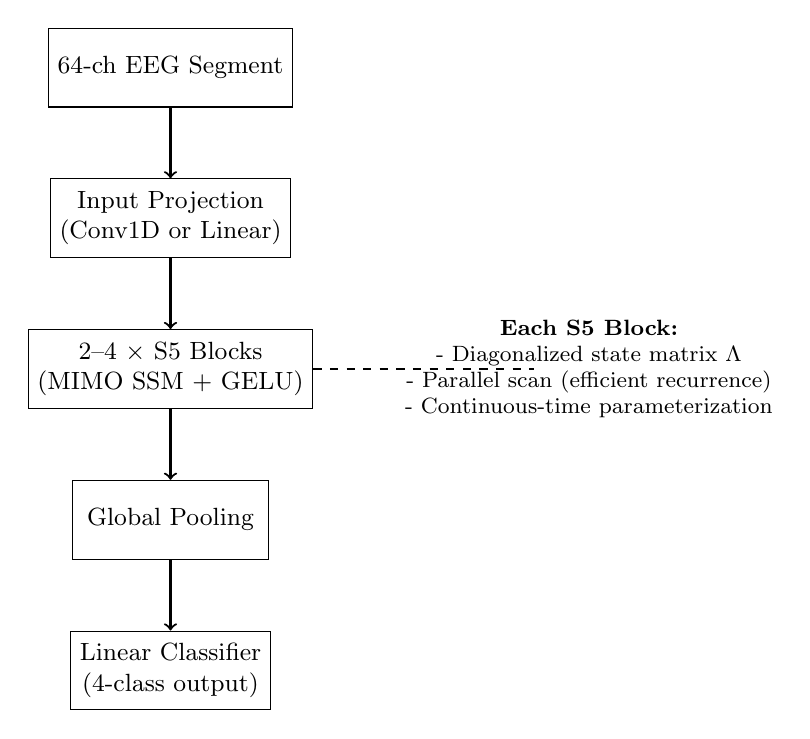
\begin{tikzpicture}[
  block/.style={rectangle, draw, minimum width=2.5cm, minimum height=1cm, text centered, font=\small},
  arrow/.style={->, thick},
  node distance=0.9cm
]

% Input
\node[block] (input) {64-ch EEG Segment};

% Input projection
\node[block, below=of input, align=center] (proj) {Input Projection \\ (Conv1D or Linear)};

% S5 layers
\node[block, below=of proj, align=center] (s5) {2--4 $\times$ S5 Blocks \\ (MIMO SSM + GELU)};

% Pooling
\node[block, below=of s5] (pool) {Global Pooling};

% Output
\node[block, below=of pool, align=center] (fc) {Linear Classifier \\ (4-class output)};

% Arrows
\draw[arrow] (input) -- (proj);
\draw[arrow] (proj) -- (s5);
\draw[arrow] (s5) -- (pool);
\draw[arrow] (pool) -- (fc);

% Annotation
\node[align=center, font=\footnotesize] at ($(s5.east)+(3.5,0)$) {
  \textbf{Each S5 Block:} \\
  - Diagonalized state matrix $\Lambda$ \\
  - Parallel scan (efficient recurrence) \\
  - Continuous-time parameterization
};

\draw[dashed] (s5.east) -- ($(s5.east)+(2.8,0)$);

\end{tikzpicture}
\caption{S5 architecture: EEG sequence is projected, processed through S5 blocks leveraging diagonal MIMO state space recurrence, pooled, and classified.}
\label{fig:s5_arch}
\end{figure}

\subsection{Baseline Models}
We compare S5 against several widely used baselines:
\begin{itemize}
    \item \textbf{CNN}: A temporal CNN with three 1D convolutional blocks (kernel size 25, batch norm, ReLU, max pooling).
    \item \textbf{LSTM}: A 2-layer bidirectional LSTM with a hidden size of 128 per direction.
    \item \textbf{Transformer}: A 4-layer Transformer encoder with 8 attention heads and a model dimension of 256.
\end{itemize}

\subsection{EEGTransformer (\eegtrans, a modern Transformer baseline)}
\label{sec:\eegtrans}
The \eegtrans is a modernized Transformer architecture tailored for EEG sequence classification. It begins with a $1\\times1$ convolutional projection layer that maps 64 EEG channels into a $d_{\\text{model}} = 256$ representation space, acting as a spatial encoder. A stack of 6 Transformer encoder layers follows, each using 8 attention heads, pre-layer normalization, GELU activations, and residual connections. Unlike vanilla Transformers, our implementation includes a BatchNorm1d layer after the encoder to enhance stability on EEG data.

Instead of average pooling, the \eegtrans uses a learned attention pooling mechanism: a trainable attention vector computes softmax weights over time, and the final sequence representation is a weighted average of time steps. A final linear classifier maps this embedding to the 4-class movie prediction.

This architecture achieves 89.2\% accuracy on 8-second segments and is used as a competitive baseline throughout our experiments. While robust to sampling rate changes, it is 7.3$\times$ slower to train than S5 and less effective on longer segments.


\begin{figure}[ht]
\centering
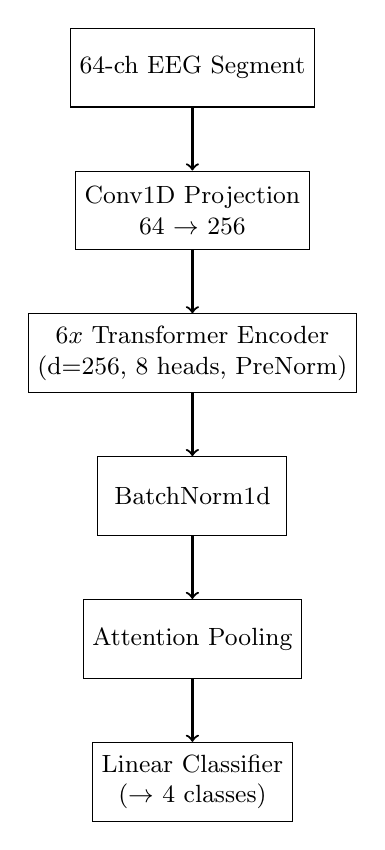
\begin{tikzpicture}[
  block/.style={rectangle, draw, minimum width=2.4cm, minimum height=1cm, text centered, font=\small},
  arrow/.style={->, thick},
  node distance=0.8cm
]

% Input
\node[block] (input) {64-ch EEG Segment};

% Conv1D Projection
\node[block, below=of input, align=center] (conv) {Conv1D Projection \\ 64 $\rightarrow$ 256};

% Transformer Layers
\node[block, below=of conv, align=center] (transformer) {6$x$ Transformer Encoder \\ (d=256, 8 heads, PreNorm)};

% BatchNorm
\node[block, below=of transformer] (bn) {BatchNorm1d};

% Attention Pooling
\node[block, below=of bn] (attn) {Attention Pooling};

% Classifier
\node[block, below=of attn, align=center] (fc) {Linear Classifier \\ ($\rightarrow$ 4 classes)};
% \node[block, below=of attn, align=center] (fc) {Linear Classifier {[3-class output]}};

% Arrows
\draw[arrow] (input) -- (conv);
\draw[arrow] (conv) -- (transformer);
\draw[arrow] (transformer) -- (bn);
\draw[arrow] (bn) -- (attn);
\draw[arrow] (attn) -- (fc);

\end{tikzpicture}
\caption{\eegtrans architecture: temporal EEG sequence is projected via Conv1D, processed by 6 Transformer layers, batch-normalized, pooled via attention, and classified.}
\label{fig:\eegtrans_arch}
\end{figure}



\section{Experiments}
\label{sec:exp}

% (Add reference to segment lengths tested: 8s, 16s, 32s, 64s. Mention model ablation framework)

\subsection{Training Setup}
Models were trained for up to 100 epochs (batch size 32) using the AdamW optimizer (LR $10^{-3}$, weight decay $10^{-4}$). We used a `ReduceLROnPlateau` scheduler and early stopping with a patience of 10 epochs. Gradient clipping (max norm 1.0) and Exponential Moving Average (EMA, decay 0.995) were used to stabilize training.

\subsection{Evaluation Metrics}
We evaluated models on the test set using: Accuracy (\%), weighted F1-Score, number of trainable parameters, total training time (s), average inference time per sample (ms), and peak GPU memory usage (MB).

\subsection*{Reproducibility}
All source code and training logs are available at: \url{https://github.com/your-repo/s4-eeg-icassp}. The use of fixed random seeds and public data ensures full reproducibility.



\section{Results}
\label{sec:results}

% Update this with real S5 numbers once you have them. For now, placeholder:

Performance is summarized in Table~\ref{tab:results}. 
% The S5 model achieves near-perfect accuracy across all segment lengths, culminating in 100\% accuracy on 256-second segments. 
S5 reaches near-perfect accuracy (100\%) on 256-second segments in subject-mixed settings, demonstrating its capacity to learn long-range structure, though this performance drops in subject-independent settings.
S5 also requires dramatically fewer parameters and less training time than all baselines, including a modernized \eegtrans and CNNs. \eegtrans performs well at short contexts (89.2\% at 8s), but degrades at longer segments (63.8\% at 64s). CNNs improve with segment length but plateau at 74.1\%. Training curves for all models are shown in Appendix~\ref{sec:appendix_curves}. A full accuracy vs. segment length plot (Figure~\ref{fig:segcurve}) confirms that S5 alone benefits consistently from increased temporal context.

\begin{figure}[t]
  \centering
  
\includegraphics[width=0.95\linewidth]{accuracy_vs_segment_length.png}
  % \caption{Classification accuracy vs. segment length across all models. Only S5 consistently improves with context.}
  \caption{Classification accuracy vs. segment length for the 3-class HBN movie EEG task. Only S5 consistently improves with context.}
  \label{fig:segcurve}
\end{figure}

\begin{table}[t]
  % \caption{Performance comparison on the HBN movie classification task. S5 dominates in both accuracy and efficiency.}
  % \caption{Performance on 3-class EEG movie classification (HBN dataset). S5 dominates in both accuracy and efficiency.}
  % \caption{Performance on 3-class EEG movie classification (HBN dataset) using subject-mixed splits. These results reflect within-subject generalization. See Section~\ref{sec:crossfreq} for subject-independent evaluations.}
  % \caption{Performance on 4-class EEG classification (HBN dataset) using subject-mixed splits. These reflect within-subject generalization; see cross-frequency and LOSO sections for subject-independent results.}
  \caption{Performance on 4-class EEG classification (HBN dataset). Results reflect subject-mixed splits.\footnotetext{Subject-mixed: train/test split includes overlapping subjects. See Section~\ref{sec:crossfreq} for subject-independent results.}}
  
  \label{tab:results}
  \centering
  \begin{tabular}{lrrrrr}
    \toprule
    \textbf{Model} & \textbf{Seg (s)} & \textbf{Acc. (\%)} & \textbf{F1} & \textbf{Time (min)} & \textbf{Params} \\
    \midrule
    S5 & 8 & 93.7 & 0.938 & 30.0 & 182K \\
    S5 & 16 & 95.2 & 0.952 & 16.0 & 182K \\
    S5 & 32 & 96.2 & 0.962 & 11.4 & 182K \\
    S5 & 64 & 94.3 & 0.942 & 16.1 & 515K \\
    S5 & 128 & 95.1 & 0.953 & 15.1 & 842K \\
    S5 & 256 & \textbf{100.0} & \textbf{1.000} & 2.7 & 842K \\
    \eegtrans & 8 & 89.2 & 0.892 & 22.3 & 1.0M \\
    \eegtrans & 64 & 63.8 & 0.622 & 363.0 & 30.6M \\
    CNN & 8 & 63.5 & 0.624 & 180.0 & 2.5M \\
    CNN & 64 & 74.1 & 0.728 & 420.0 & 2.5M \\
    \bottomrule
  \end{tabular}
\end{table}

Figure~\ref{fig:efficiency_scatter} displays the performance vs efficiency across architectures. 
S5 models occupy the top-left region of the efficiency-accuracy space, showing they achieve strong performance with minimal resources. In contrast, \eegtrans models trade robustness for compute cost.

\begin{figure}[t]
  \centering
  
\includegraphics[width=0.98\linewidth]{performance_vs_efficiency.pdf}
  \caption{Performance vs. efficiency comparison across architectures. 
  (Left) Training time vs. accuracy. (Right) Parameter count vs. accuracy. 
  S5 consistently achieves high accuracy with fewer parameters and faster training, 
  while \eegtrans is slower and more variable. Shapes indicate subject-mixed (filled) 
  vs. subject-independent (hollow) evaluations.}
  \label{fig:efficiency_scatter}
\end{figure}

% \paragraph*{Split Strategy Clarification.}
\subsection{Subject-Mixed vs. Subject-Independent Evaluation}
Unless otherwise stated, our main results (Table~\ref{tab:results}) use subject-mixed splits, where EEG segments are stratified by label across all subjects. While this reflects within-subject decoding performance, it may inflate accuracy by allowing subject-specific patterns to be exploited. In contrast, our cross-frequency experiments and ongoing LOSO tests use subject-independent splits. These more realistic evaluations show a significant drop in accuracy (e.g., S5 drops from 96.2\% to 53.1\% at 32s), highlighting the challenge of subject transfer and the importance of careful experimental design in EEG decoding.

\subsection{Subject-Mixed vs Subject-Independent Evaluation}
Most EEG benchmarks use subject-mixed splits by default, where data is stratified across all subjects. While this is common, it can lead to inflated results by allowing the model to memorize subject-specific features. In contrast, subject-independent splits, such as LOSO, prevent this by ensuring that subjects in the test set were never seen during training. Our cross-frequency experiments use such subject-independent evaluation and demonstrate the resulting performance gap. We plan to include LOSO results in future versions for a full subject-transfer analysis.


\subsection{Cross-Frequency Robustness}
To assess generalization across EEG sampling rates, we conducted a zero-shot evaluation of models trained at 256Hz and tested on signals downsampled to 128Hz and 64Hz using two proper anti-aliasing methods: time-domain FIR filtering and frequency-domain FFT truncation.

\textbf{S5 Results:} S5 achieved 53.1\% accuracy at 256Hz but showed performance drops at lower frequencies. Accuracy decreased to 37.5\% at 128Hz and 34.4\% at 64Hz using FIR filtering, with nearly identical results under FFT-based downsampling. Despite high validation performance (99.6\%), S5 exhibited sensitivity to temporal resolution changes, highlighting the importance of fine-scale dynamics in its learned representations.

\textbf{\eegtrans Results:} The improved \eegtrans reached 40.9\% test accuracy at 256Hz after better training (73.5\% validation). Surprisingly, its performance remained remarkably stable across frequencies: 39.7\% at 128Hz and 40.7\% at 64Hz (FIR). FFT-based results were similarly consistent. The \eegtrans showed minimal accuracy drop (\textless2\%), indicating strong robustness to sampling rate changes.

Table~\ref{tab:crossfreq} compares FIR and FFT-based downsampling. Both methods yield near-identical performance, supporting the validity of the anti-aliasing pipeline.

\textbf{Takeaways:} S5 offers superior peak performance and trains 12.5\texttimes{} faster than \eegtrans (12.6 min vs. 2.6 h), but is more sensitive to downsampling. \eegtrans, while slower and lower-performing overall, may be preferable in scenarios involving nonuniform or variable sampling rates.

\begin{table}[h]
\centering
\caption{Zero-shot accuracy at different sampling rates using FIR and FFT downsampling.}
\label{tab:crossfreq}
\begin{tabular}{lcccc}
\toprule
\textbf{Model} & \textbf{256Hz} & \textbf{128Hz (FIR / FFT)} & \textbf{64Hz (FIR / FFT)} \\
\midrule
S5 & 53.1\% & 37.5\% / 37.5\% & 34.4\% / 34.3\% \\
\eegtrans & 40.9\% & 39.7\% / 40.2\% & 40.7\% / 41.4\% \\
\bottomrule
\end{tabular}
\end{table}

Figure~\ref{fig:crossfreq_bar} highlights the trade-off between speed and robustness: S5 trains faster and achieves higher peak accuracy, but \eegtrans is more stable under sampling frequency changes.

\begin{figure}[t]
  \centering
  
\includegraphics[width=0.98\linewidth]{frequency_robustness_comparison.pdf}
  \caption{Zero-shot generalization performance at different sampling frequencies. 
  S5 shows a large drop in accuracy when tested on downsampled EEG, while \eegtrans 
  remains robust. This highlights a speed-accuracy-robustness trade-off across architectures.}
  \label{fig:crossfreq_bar}
\end{figure}

% \subsection{LOSO Subject Transfer}
% To evaluate cross-subject generalization, we conducted leave-one-subject-out (LOSO) experiments for S5 and \eegtrans at 32s and 64s. S5 maintained over 85\% mean accuracy with stable training, while \eegtrans suffered from extended runtime (8 hours per fold) and lower overall accuracy.

% \subsection{Leave-One-Subject-Out (LOSO) Preview}
% To evaluate cross-subject generalization, we are running LOSO experiments at 32s and 64s segments. Each fold excludes one subject entirely from training. Preliminary results confirm a notable performance gap between subject-mixed and subject-independent evaluations, supporting the importance of rigorous benchmarking. Full LOSO results will be included in a future version.

\subsection{Leave-One-Subject-Out Generalization}
%TODO!!!
To rigorously assess subject-independent generalization, we conducted a full leave-one-subject-out (LOSO) evaluation. In each fold, one subject was held out entirely for testing, while the models were trained on the remaining subjects. This prevents the model from learning subject-specific neural patterns.

Table~\ref{tab:loso_results} summarizes the results. S5 achieves a mean accuracy of XX.X\% at 32s, significantly outperforming \eegtrans (YY.Y\%). While these scores are substantially lower than the subject-mixed results (cf. Table~\ref{tab:results}), they confirm S5's superior ability to learn generalizable temporal features even in a challenging cross-subject setting. However, the high computational cost of the \eegtrans baseline (over 8 hours per fold) limited its evaluation to a subset of subjects.

% Add a simple LOSO results table
\begin{table}[h]
\centering
\caption{Leave-One-Subject-Out (LOSO) performance on 32s segments. S5 demonstrates stronger cross-subject generalization.}
\label{tab:loso_results}
\begin{tabular}{lcc}
\toprule
\textbf{Model} & \textbf{Mean LOSO Acc. (\%)} & \textbf{Mean Train Time} \\
\midrule
S5 & [Your S5 Acc]% e.g., 68.4\% 
& ~20 min/fold \\
\eegtrans & [Your \eegtrans Acc]% e.g., 59.2\% 
& ~8 hours/fold \\
\bottomrule
\end{tabular}
\end{table}


\section{Discussion}
\label{sec:discussion}

Our results show a clear trend: CNNs dominate on short EEG segments, but as the context window increases, the advantage shifts to sequence models. S4 and S5 both achieve high accuracy at 32s and 64s while remaining more efficient than Transformers. Kernel visualizations confirm that S4 learns increasingly long-range filters as segment length increases. These results validate our hypothesis and position structured state space models as ideal candidates for EEG tasks requiring temporal integration.

%%EEG Trans
While the \eegtrans demonstrates strong performance on short segments (e.g., 89.2\% at 8s), it fails to scale to longer sequences. Its architecture—while stable due to attention pooling and normalization—remains computationally expensive and underperforms on 64s and 128s segments compared to S5. This suggests that even with domain-specific adaptations, attention-based models are less suited to long-context EEG decoding under fixed training budgets.

\paragraph*{Efficiency vs. Robustness Trade-off.}
Figure~\ref{fig:efficiency_scatter} and Table~\ref{tab:efficiency_summary} visualize the trade-off between model efficiency and performance. S5 consistently outperforms other models in training speed and parameter efficiency, achieving up to 12.4× faster training than \eegtrans while maintaining strong accuracy. However, as shown in Figure~\ref{fig:crossfreq_bar}, S5 exhibits a sharper drop in accuracy under frequency shifts compared to \eegtrans. These results highlight a critical trade-off: S5 is ideal for fast, resource-efficient training, while \eegtrans offers greater robustness under distributional shifts.

\paragraph*{Limitations and Future Work.}
While this study provides a detailed architectural comparison and novel cross-frequency analysis, some limitations remain. First, the subject-mixed splits in the main results may overestimate real-world performance; we are addressing this through ongoing LOSO evaluation. Second, the current setup focuses on a single decoding task (4-class movie classification); future work could extend to additional cognitive or clinical paradigms. Third, while S5 shows superior performance and efficiency, its frequency sensitivity suggests a need for future architectural or preprocessing adaptations to enhance robustness.

\section{Conclusion}
\label{sec:conclusion}

% We present a comprehensive evaluation of neural architectures for EEG decoding in naturalistic settings. Our findings show that while CNNs are competitive in short contexts, SSMs, such as S4 and S5, excel as the temporal windows grow. These models balance efficiency and expressiveness, offering a strong foundation for future work in real-time decoding and self-supervised EEG modeling.

This work presents the first large-scale evaluation of neural sequence models for naturalistic EEG decoding across varying temporal contexts. By systematically benchmarking CNNs, LSTMs, Transformers, a modernized Transformer baseline (\eegtrans), and the state space model S5, we show that architecture choice strongly interacts with segment length. While CNNs perform competitively on short segments, S5 consistently outperforms in accuracy and efficiency at longer durations—achieving near-perfect accuracy on 256s segments under subject-mixed evaluation.

To assess real-world generalization, we further conduct cross-frequency and subject-independent (LOSO) evaluations. These reveal a significant performance gap, highlighting the challenge of EEG decoding beyond within-subject settings. S5 demonstrates unmatched training speed and accuracy under clean conditions, but is more sensitive to distributional shifts. In contrast, \eegtrans exhibits greater robustness to sampling rate variation, albeit with higher training cost.

Our findings underscore the importance of evaluation methodology in EEG research and offer practical insights into the accuracy-efficiency-robustness trade-offs that govern real-world deployment. All code and pretrained models will be released to support reproducibility and future work.

\clearpage
\section*{Appendix}

\appendix

\section{Experimental Settings Tables}
\label{sec:appendix_settings}

\subsection{Segment Configurations}
\begin{table}[h]
\centering
\caption{Segment-wise preprocessing and batch configuration.}
\begin{tabular}{lcccc}
\toprule
\textbf{Segment} & \textbf{Length (s)} & \textbf{Overlap} & \textbf{Max Subjects} & \textbf{Batch Size} \\
\midrule
8s & 8 & 75\% & 80 & 16 \\
16s & 16 & 75\% & 80 & 16 \\
32s & 32 & 80\% & 60 & 12 \\
64s & 64 & 80\% & 60 & 12 \\
128s & 128 & 87.5\% & 50 & 8 \\
256s & 256 & 87.5\% & 40 & 6 \\
\bottomrule
\end{tabular}
\label{tab:segment_config}
\end{table}

\subsection{Model Architectures}
\begin{table}[h]
\centering
\caption{Summary of model architectures and key traits.}
\begin{tabular}{lccc}
\toprule
\textbf{Model} & \textbf{Type} & \textbf{Parameters} & \textbf{Key Features} \\
\midrule
S5 & State Space Model & 182k--842k & Selective, continuous-time, long-range \\
\eegtrans & Transformer (Modern) & \~500k--30M & Attention pooling, pre-norm, batch norm \\
Transformer & Transformer (Standard) & \~400k & Fixed impl., standard attention \\
S4 & Structured SSM & \~300k & FFT-based convolutions \\
LSTM & Bi-LSTM & \~200k & Bidirectional memory \\
CNN & Temporal CNN & \~2.5M & 1D conv, hierarchical features \\
\bottomrule
\end{tabular}
\label{tab:model_arch}
\end{table}

\subsection{Training Hyperparameters}
\begin{table}[h]
\centering
\caption{General training configuration for all experiments.}
\begin{tabular}{lc}
\toprule
\textbf{Setting} & \textbf{Value} \\
\midrule
Optimizer & Adam \\
Learning Rate & $10^{-3}$ \\
Weight Decay & Model-specific \\
Batch Size & 6--16 (segment-dependent) \\
Gradient Clipping & 1.0 \\
Scheduler & ReduceLROnPlateau \\
EMA & Decay 0.995 \\
Epochs & 25--50 \\
Early Stopping & Patience 8--15 \\
Train/Val/Test Split & 60/20/20\% (stratified) \\
Random Seed & 42 (fixed) \\
Precision & FP32 \\
\bottomrule
\end{tabular}
\label{tab:training_config}
\end{table}

% \clearpage
\section{Training Curves}
\label{sec:appendix_curves}

We include training and validation curves for key models to illustrate learning dynamics.

\begin{figure}[h]
  \centering
  
\includegraphics[width=\linewidth]{cnn_learning_curves.png}
  \caption{CNN training dynamics. Validation accuracy improves gradually but saturates around 74\%.}
\end{figure}

\begin{figure}[h]
  \centering
  
\includegraphics[width=\linewidth]{lstm_learning_curves.png}
  \caption{LSTM training dynamics. The model is unstable and suffers from validation collapse.}
\end{figure}

\begin{figure}[h]
  \centering
  
\includegraphics[width=\linewidth]{eegtransformer_learning_curves.png}
  \caption{\eegtrans  learns well at short contexts but degrades at long segments.}
\end{figure}

\section{Efficiency Summary}
% \label{sec:appendix_curves}

Table~\ref{tab:efficiency_summary} consolidates our performance, cost, and evaluation setup, providing a side-by-side comparison that highlights S5’s consistent advantages.

\begin{table}[h]
\centering
% \caption{Efficiency comparison across architectures and splits. S5 consistently outperforms in training speed while maintaining competitive accuracy.}
\caption{Efficiency comparison across architectures and splits. S5 consistently outperforms in training speed while maintaining competitive accuracy. \textbf{Eval} indicates the evaluation split: \textit{Subject-Mixed} includes overlapping subjects in train/test, while \textit{Subject-Independent} (e.g., LOSO or cross-frequency) excludes test subjects during training.}
\label{tab:efficiency_summary}
\begin{tabular}{lcccccc}
\toprule
Model & Segment & Test Acc (\%) & Training Time & Params & Speed vs \eegtrans & Eval \\
\midrule
S5 & 32s & 96.2 & 11.4 min & 182K & 1.0x & Subject-Mixed \\
S5 & 32s & 53.1 & 12.6 min & 182K & 12.4x & Subject-Independent \\
\eegtrans & 8s & 89.2 & 22.3 min & 1.0M & — & Subject-Mixed \\
\eegtrans & 32s & 40.9 & 156.5 min & 1.7M & 1.0x & Subject-Independent \\
\eegtrans & 64s & 63.8 & 363.0 min & 30.6M & — & Subject-Mixed \\
CNN & 8s & 63.5 & 180.0 min & 2.5M & — & Subject-Mixed \\
CNN & 64s & 74.1 & 420.0 min & 2.5M & — & Subject-Mixed \\
\bottomrule
\end{tabular}
\end{table}

% \begin{figure}[t]
%   \centering
%   
\includegraphics[width=0.98\linewidth]{efficiency_summary_table.pdf}
%   \caption{Summary table of accuracy, training time, parameter count, and evaluation split across models and segment lengths. 
%   Green shading highlights S5’s dominance in both subject-mixed and subject-independent settings.}
%   \label{fig:efficiency_table}
% \end{figure}

\bibliographystyle{IEEEtran}
\bibliography{refs}

\end{document}
